\documentclass[]{tufte-handout}

% ams
\usepackage{amssymb,amsmath}

\usepackage{ifxetex,ifluatex}
\usepackage{fixltx2e} % provides \textsubscript
\ifnum 0\ifxetex 1\fi\ifluatex 1\fi=0 % if pdftex
  \usepackage[T1]{fontenc}
  \usepackage[utf8]{inputenc}
\else % if luatex or xelatex
  \makeatletter
  \@ifpackageloaded{fontspec}{}{\usepackage{fontspec}}
  \makeatother
  \defaultfontfeatures{Ligatures=TeX,Scale=MatchLowercase}
  \makeatletter
  \@ifpackageloaded{soul}{
     \renewcommand\allcapsspacing[1]{{\addfontfeature{LetterSpace=15}#1}}
     \renewcommand\smallcapsspacing[1]{{\addfontfeature{LetterSpace=10}#1}}
   }{}
  \makeatother

\fi

% graphix
\usepackage{graphicx}
\setkeys{Gin}{width=\linewidth,totalheight=\textheight,keepaspectratio}

% booktabs
\usepackage{booktabs}

% url
\usepackage{url}

% hyperref
\usepackage{hyperref}

% units.
\usepackage{units}


\setcounter{secnumdepth}{-1}

% citations
\usepackage{natbib}
\bibliographystyle{plainnat}


% pandoc syntax highlighting
\usepackage{color}
\usepackage{fancyvrb}
\newcommand{\VerbBar}{|}
\newcommand{\VERB}{\Verb[commandchars=\\\{\}]}
\DefineVerbatimEnvironment{Highlighting}{Verbatim}{commandchars=\\\{\}}
% Add ',fontsize=\small' for more characters per line
\newenvironment{Shaded}{}{}
\newcommand{\AlertTok}[1]{\textcolor[rgb]{1.00,0.00,0.00}{\textbf{#1}}}
\newcommand{\AnnotationTok}[1]{\textcolor[rgb]{0.38,0.63,0.69}{\textbf{\textit{#1}}}}
\newcommand{\AttributeTok}[1]{\textcolor[rgb]{0.49,0.56,0.16}{#1}}
\newcommand{\BaseNTok}[1]{\textcolor[rgb]{0.25,0.63,0.44}{#1}}
\newcommand{\BuiltInTok}[1]{#1}
\newcommand{\CharTok}[1]{\textcolor[rgb]{0.25,0.44,0.63}{#1}}
\newcommand{\CommentTok}[1]{\textcolor[rgb]{0.38,0.63,0.69}{\textit{#1}}}
\newcommand{\CommentVarTok}[1]{\textcolor[rgb]{0.38,0.63,0.69}{\textbf{\textit{#1}}}}
\newcommand{\ConstantTok}[1]{\textcolor[rgb]{0.53,0.00,0.00}{#1}}
\newcommand{\ControlFlowTok}[1]{\textcolor[rgb]{0.00,0.44,0.13}{\textbf{#1}}}
\newcommand{\DataTypeTok}[1]{\textcolor[rgb]{0.56,0.13,0.00}{#1}}
\newcommand{\DecValTok}[1]{\textcolor[rgb]{0.25,0.63,0.44}{#1}}
\newcommand{\DocumentationTok}[1]{\textcolor[rgb]{0.73,0.13,0.13}{\textit{#1}}}
\newcommand{\ErrorTok}[1]{\textcolor[rgb]{1.00,0.00,0.00}{\textbf{#1}}}
\newcommand{\ExtensionTok}[1]{#1}
\newcommand{\FloatTok}[1]{\textcolor[rgb]{0.25,0.63,0.44}{#1}}
\newcommand{\FunctionTok}[1]{\textcolor[rgb]{0.02,0.16,0.49}{#1}}
\newcommand{\ImportTok}[1]{#1}
\newcommand{\InformationTok}[1]{\textcolor[rgb]{0.38,0.63,0.69}{\textbf{\textit{#1}}}}
\newcommand{\KeywordTok}[1]{\textcolor[rgb]{0.00,0.44,0.13}{\textbf{#1}}}
\newcommand{\NormalTok}[1]{#1}
\newcommand{\OperatorTok}[1]{\textcolor[rgb]{0.40,0.40,0.40}{#1}}
\newcommand{\OtherTok}[1]{\textcolor[rgb]{0.00,0.44,0.13}{#1}}
\newcommand{\PreprocessorTok}[1]{\textcolor[rgb]{0.74,0.48,0.00}{#1}}
\newcommand{\RegionMarkerTok}[1]{#1}
\newcommand{\SpecialCharTok}[1]{\textcolor[rgb]{0.25,0.44,0.63}{#1}}
\newcommand{\SpecialStringTok}[1]{\textcolor[rgb]{0.73,0.40,0.53}{#1}}
\newcommand{\StringTok}[1]{\textcolor[rgb]{0.25,0.44,0.63}{#1}}
\newcommand{\VariableTok}[1]{\textcolor[rgb]{0.10,0.09,0.49}{#1}}
\newcommand{\VerbatimStringTok}[1]{\textcolor[rgb]{0.25,0.44,0.63}{#1}}
\newcommand{\WarningTok}[1]{\textcolor[rgb]{0.38,0.63,0.69}{\textbf{\textit{#1}}}}

% table with pandoc

% multiplecol
\usepackage{multicol}

% strikeout
\usepackage[normalem]{ulem}

% morefloats
\usepackage{morefloats}


% tightlist macro required by pandoc >= 1.14
\providecommand{\tightlist}{%
  \setlength{\itemsep}{0pt}\setlength{\parskip}{0pt}}

% title / author / date
\title[Análise mamíferos terrestres -- 2017 a 2021]{Encontro dos Saberes
RESEX do Rio Ouro Preto (2022)}
\author{Elildo Carvalho Jr - ICMBio/CENAP}
\date{2022-03-28}

\usepackage{booktabs}
\usepackage{longtable}
\usepackage{array}
\usepackage{multirow}
\usepackage{wrapfig}
\usepackage{float}
\usepackage{colortbl}
\usepackage{pdflscape}
\usepackage{tabu}
\usepackage{threeparttable}
\usepackage{threeparttablex}
\usepackage[normalem]{ulem}
\usepackage{makecell}
\usepackage{xcolor}

\begin{document}

\maketitle




\begin{verbatim}
## # A tibble: 632 x 13
##    nome_UC        estacao_amostral nome_ea esforco data         ano classe ordem
##    <chr>                     <dbl> <chr>     <dbl> <date>     <dbl> <chr>  <chr>
##  1 Resex do Rio ~                1 Franci~    3650 2017-06-03  2017 Mamma~ Prim~
##  2 Resex do Rio ~                1 Franci~      NA 2017-06-03  2017 Mamma~ Prim~
##  3 Resex do Rio ~                1 Franci~      NA 2017-06-03  2017 Mamma~ Rode~
##  4 Resex do Rio ~                1 Franci~    3650 2017-06-04  2017 Aves   Tina~
##  5 Resex do Rio ~                1 Franci~      NA 2017-06-04  2017 Mamma~ Rode~
##  6 Resex do Rio ~                1 Franci~      NA 2017-06-04  2017 Aves   Tina~
##  7 Resex do Rio ~                1 Franci~      NA 2017-06-04  2017 Mamma~ Prim~
##  8 Resex do Rio ~                1 Franci~    3650 2017-06-05  2017 Mamma~ Prim~
##  9 Resex do Rio ~                1 Franci~      NA 2017-06-05  2017 Mamma~ Prim~
## 10 Resex do Rio ~                1 Franci~      NA 2017-06-05  2017 Aves   Gall~
## # ... with 622 more rows, and 5 more variables: familia <chr>, genero <chr>,
## #   especie <chr>, n_animais <dbl>, distancia <dbl>
\end{verbatim}

\begin{verbatim}
## # A tibble: 22 x 2
## # Groups:   especie [22]
##    especie                     n
##    <chr>                   <int>
##  1 Ateles chamek              26
##  2 Callicebus brunneus        19
##  3 Cavia fulgida               1
##  4 Cebus unicolor              5
##  5 Cerdocyon thous             2
##  6 Cuniculus paca              1
##  7 Dasyprocta fuliginosa      65
##  8 Dasyprocta sp.              1
##  9 Dasypus kappleri            1
## 10 Dasypus novemcinctus        1
## 11 Mazama americana            6
## 12 Mazama nemorivaga           9
## 13 Myrmecophaga tridactyla     1
## 14 Nasua nasua                 4
## 15 Pecari tajacu              17
## 16 Pithecia irrorata          10
## 17 Saguinus weddelli          12
## 18 Saimiri ustus              27
## 19 Sapajus apella            133
## 20 Tamandua tetradactyla       4
## 21 Tayassu pecari              5
## 22 Urosciurus spadiceus       13
\end{verbatim}

\hypertarget{apresentauxe7uxe3o}{%
\subsection{Apresentação}\label{apresentauxe7uxe3o}}

Este relatório apresenta resultados do Programa Monitora, Subprograma
Terrestre, Componente Florestal Global, Alvo Mamíferos terrestres de
médio e grande porte, protocolo básico, na \textbf{Reserva Extrativista
do Rio Ouro Preto}, 2017 a 2021. O principal objetivo é subsidiar o
Encontro dos Saberes que será realizado nesta unidade.

Por se tratar de um relatório simplificado, este documento não inclui
detalhes sobre métodos de coleta ou análise dos dados. Ele também não
inclui detalhes sobre o esforço de amostragem, pois essa informação já
consta do relatório produzido pelo CEMAVE. Portanto, o relatório apenas
apresenta as variações anuais nas populações de espécies selecionadas de
mamíferos de médio e grande porte.

\hypertarget{nuxfamero-total-de-encontros}{%
\subsection{Número total de
encontros}\label{nuxfamero-total-de-encontros}}

A tabela 1 apresenta o número total de encontros e de indivíduos
avistados por espécie, e a Figura 1 apresenta o número total de
encontros para as espécies que tiveram pelo menos 5 encontros ao longo
de todo o monitoramento.

As espécies mais encontradas foram, nessa ordem: cutia, caititu,
quatipuru e veado fuboca/mateiro. As outras espécies foram encontradas
poucas vezes. Algumas espécies vivem em grupos, por isso o número
indivíduos pode ser maior do que o número de encontros. De forma geral,
as espécies com mais indivíduos foram também as mais encontradas.

É importante lembrar que só porque uma espécie foi registrada poucas
vezes, não quer dizer necessariamente que ela seja rara. Por exemplo, o
protocolo não funciona bem para espécies noturnas como as antas e as
pacas, pois as trilhas são percorridas durante o dia, quando essas
espécies estão menos ativas. Além disso, espécies que são caçadas podem
ficar muito ariscas, fugindo ao menor sinal da aproximação de pessoas.

\begin{table}

\caption{\label{tab:unnamed-chunk-2}Tabela 1. Numero de registros por especie obtidos pelo protocolo básico do Programa Monitora na Resex do Rio Ouro Preto, 2017-2021}
\centering
\begin{tabular}[t]{llllcl}
\toprule
Ordem & Familia & Especie & Nome popular & Encontros & Individuos\\
\midrule
Artiodactyla & Cervidae & Mazama americana & Veado-mateiro & 6 & 6\\
Artiodactyla & Cervidae & Mazama nemorivaga & Veado-fuboca & 9 & 11\\
Artiodactyla & Tayassuidae & Pecari tajacu & Caititu & 17 & 45\\
Artiodactyla & Tayassuidae & Tayassu pecari & Queixada & 5 & 71\\
Carnivora & Canidae & Cerdocyon thous & Raposinha & 2 & 2\\
\addlinespace
Carnivora & Procyonidae & Nasua nasua & Quati & 4 & 9\\
Cingulata & Dasypodidae & Dasypus kappleri & Tatu-quinze-quilos & 1 & 1\\
Cingulata & Dasypodidae & Dasypus novemcinctus & Tatu-galinha & 1 & 1\\
Pilosa & Myrmecophagidae & Myrmecophaga tridactyla & Tamanduá=bandeira & 1 & 1\\
Pilosa & Myrmecophagidae & Tamandua tetradactyla & Mambira & 4 & 4\\
\addlinespace
Rodentia & Caviidae & Cavia fulgida & Preá & 1 & 1\\
Rodentia & Cuniculidae & Cuniculus paca & Paca & 1 & 1\\
Rodentia & Dasyproctidae & Dasyprocta fuliginosa & Cutia & 66 & 73\\
Rodentia & Sciuridae & Urosciurus spadiceus & Quatipuru & 13 & 15\\
\bottomrule
\end{tabular}
\end{table}

\begin{figure}
\includegraphics{encontro_saberes_ouro_preto_handout_files/figure-latex/unnamed-chunk-3-1} \caption[Figura 1]{Figura 1. Número total de encontros por espécie na Resex do Rio Ouro Preto, 2014-2021. Somente espécies com mais de 5 encontros foram incluídas}\label{fig:unnamed-chunk-3}
\end{figure}

\hypertarget{tenduxeancias-populacionais}{%
\section{Tendências populacionais}\label{tenduxeancias-populacionais}}

Somente a cutia apresentou taxa de encontro anual média \textgreater{}
0.05 ind/km, o que equivale aproximadamente a um encontro a cada 20 km
percorridos (Tabela 2, Figura 1). As outras especies não tiveram número
de eoncontros suficiente para permitir uma análise de suas tendências
populacionais.

\begin{table}

\caption{\label{tab:unnamed-chunk-4}Tabela 2. Taxa de encontro anuais para as especies mais comuns de mamíferos terrestres em do Rio Ouro Preto. Somente espécies com taxa de encontro anual média > 0.05 ind/km foram incluídas}
\centering
\begin{tabular}[t]{lclclcl}
\toprule
especie & 2017 & 2018 & 2019 & 2020 & 2021 & means\\
\midrule
Dasyprocta fuliginosa & 0.07 & 0.11 & 0.12 & 0.13 & 0.03 & 0.093157\\
\bottomrule
\end{tabular}
\end{table}

\begin{verbatim}
## Compiling model graph
##    Resolving undeclared variables
##    Allocating nodes
## Graph information:
##    Observed stochastic nodes: 15
##    Unobserved stochastic nodes: 20
##    Total graph size: 99
## 
## Initializing model
## 
## Inference for Bugs model at "/home/elildojr/Documents/r/Programa-Monitora-Florestal-Global/encontro_saberes/ouro_preto/ssm.jags", fit using jags,
##  3 chains, each with 25000 iterations (first 10000 discarded), n.thin = 3
##  n.sims = 15000 iterations saved
##             mu.vect sd.vect  2.5%   25%   50%   75% 97.5% Rhat n.eff
## N.est[1,1]     0.11    0.11  0.02  0.05  0.08  0.14  0.38 1.00  4500
## N.est[2,1]     0.29    0.30  0.04  0.12  0.21  0.36  1.04 1.00  5800
## N.est[3,1]     0.01    0.01  0.00  0.00  0.01  0.01  0.03 1.00  8700
## N.est[1,2]     0.11    0.08  0.03  0.06  0.09  0.14  0.31 1.00 15000
## N.est[2,2]     0.10    0.07  0.02  0.05  0.08  0.13  0.29 1.00 15000
## N.est[3,2]     0.05    0.04  0.01  0.03  0.04  0.06  0.15 1.00 15000
## N.est[1,3]     0.09    0.06  0.02  0.05  0.07  0.11  0.23 1.00 15000
## N.est[2,3]     0.04    0.03  0.01  0.02  0.03  0.05  0.12 1.00 15000
## N.est[3,3]     0.13    0.09  0.03  0.07  0.11  0.17  0.37 1.00 15000
## N.est[1,4]     0.06    0.05  0.02  0.03  0.05  0.08  0.19 1.00 15000
## N.est[2,4]     0.01    0.01  0.00  0.00  0.01  0.01  0.02 1.00 15000
## N.est[3,4]     0.22    0.15  0.05  0.12  0.18  0.28  0.61 1.00 15000
## N.est[1,5]     0.04    0.04  0.01  0.02  0.03  0.05  0.14 1.00 15000
## N.est[2,5]     0.00    0.00  0.00  0.00  0.00  0.00  0.00 1.00  3400
## N.est[3,5]     0.27    0.25  0.04  0.11  0.19  0.33  0.96 1.00 14000
## mean.r[1]     -0.25    0.53 -1.29 -0.60 -0.25  0.11  0.81 1.00  5800
## mean.r[2]     -1.81    0.53 -2.87 -2.17 -1.81 -1.45 -0.76 1.00  2300
## mean.r[3]      0.85    0.54 -0.20  0.50  0.85  1.21  1.90 1.00  9900
## mean_N[1]      0.14    0.11  0.03  0.07  0.11  0.17  0.40 1.00 15000
## mean_N[2]      0.09    0.04  0.04  0.06  0.08  0.11  0.18 1.00 15000
## mean_N[3]      0.09    0.04  0.04  0.06  0.08  0.11  0.18 1.00 15000
## mean_N[4]      0.10    0.05  0.03  0.06  0.09  0.12  0.23 1.00 14000
## mean_N[5]      0.10    0.09  0.02  0.05  0.08  0.13  0.33 1.00 14000
## r[1,1]         0.13    0.74 -1.32 -0.36  0.13  0.63  1.58 1.00  2800
## r[2,1]        -0.93    0.74 -2.38 -1.44 -0.94 -0.42  0.53 1.00  3900
## r[3,1]         1.88    0.76  0.43  1.35  1.87  2.41  3.40 1.00 10000
## r[1,2]        -0.25    0.68 -1.59 -0.70 -0.25  0.20  1.09 1.00 15000
## r[2,2]        -0.87    0.70 -2.23 -1.36 -0.88 -0.39  0.52 1.00 15000
## r[3,2]         0.98    0.68 -0.36  0.53  0.97  1.42  2.31 1.00 15000
## r[1,3]        -0.30    0.68 -1.64 -0.76 -0.30  0.15  1.04 1.00 15000
## r[2,3]        -1.82    0.67 -3.12 -2.27 -1.81 -1.38 -0.48 1.00 15000
## r[3,3]         0.48    0.67 -0.85  0.02  0.49  0.93  1.79 1.00 15000
## r[1,4]        -0.57    0.74 -2.04 -1.06 -0.56 -0.06  0.87 1.00 15000
## r[2,4]        -3.64    0.86 -5.30 -4.22 -3.64 -3.06 -1.94 1.00  5900
## r[3,4]         0.07    0.76 -1.42 -0.44  0.08  0.59  1.55 1.00 15000
## sigma2.obs     0.86    0.12  0.54  0.79  0.89  0.95  1.00 1.00 12000
## sigma2.proc    0.77    0.20  0.25  0.68  0.83  0.93  0.99 1.02  1200
## deviance      50.82    7.13 38.20 45.88 50.36 55.25 66.10 1.00  3800
## 
## For each parameter, n.eff is a crude measure of effective sample size,
## and Rhat is the potential scale reduction factor (at convergence, Rhat=1).
## 
## DIC info (using the rule, pD = var(deviance)/2)
## pD = 25.4 and DIC = 76.3
## DIC is an estimate of expected predictive error (lower deviance is better).
\end{verbatim}

\begin{Shaded}
\begin{Highlighting}[]
\FunctionTok{include\_graphics}\NormalTok{(}\FunctionTok{here}\NormalTok{(}\StringTok{"encontro\_saberes"}\NormalTok{, }\StringTok{"ouro\_preto"}\NormalTok{, }\StringTok{"Dasyprocta fuliginosa 2017 a 2021.jpeg"}\NormalTok{))}
\end{Highlighting}
\end{Shaded}

\begin{verbatim}
## Warning in include_graphics(here("encontro_saberes", "ouro_preto", "Dasyprocta
## fuliginosa 2017 a 2021.jpeg")): It is highly recommended to use relative paths
## for images. You had absolute paths: "/home/elildojr/Documents/r/Programa-
## Monitora-Florestal-Global/encontro_saberes/ouro_preto/Dasyprocta fuliginosa 2017
## a 2021.jpeg"
\end{verbatim}

\begin{figure}
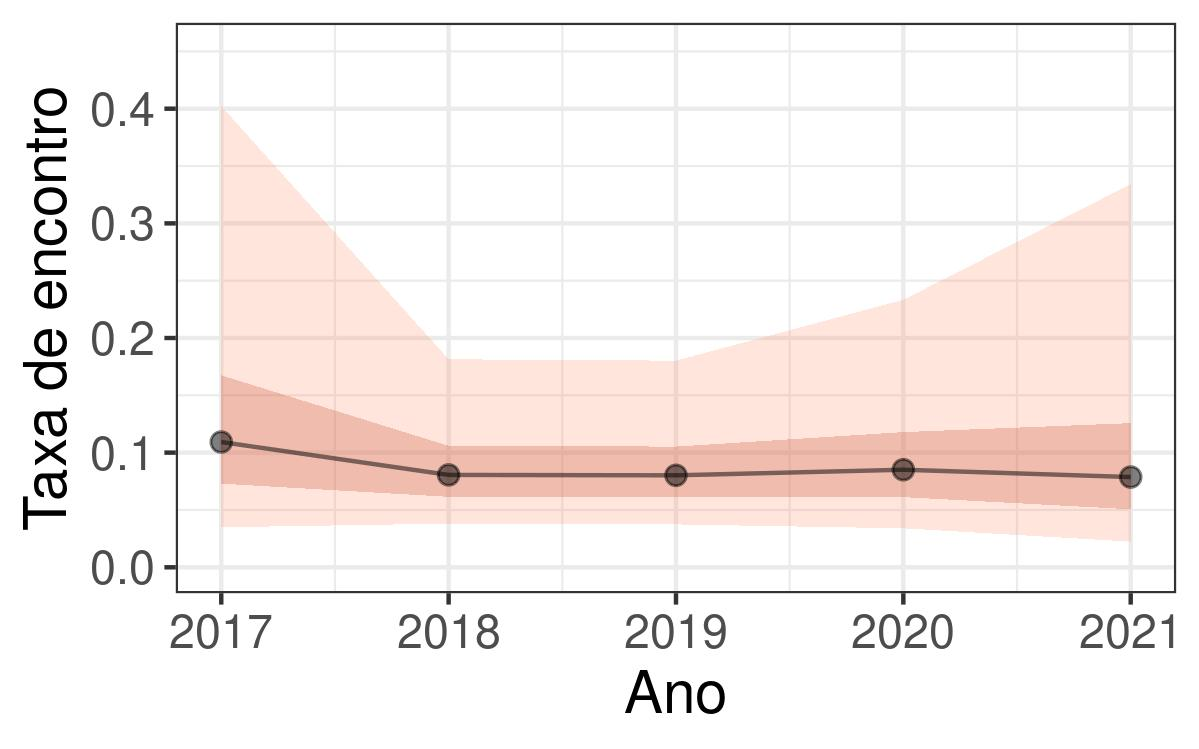
\includegraphics[width=16.65in]{/home/elildojr/Documents/r/Programa-Monitora-Florestal-Global/encontro_saberes/ouro_preto/Dasyprocta fuliginosa 2017 a 2021} \caption[Taxa de encontro anual para cutia na Resex do Rio Ouro_Preto, 2017-2021]{Taxa de encontro anual para cutia na Resex do Rio Ouro_Preto, 2017-2021}\label{fig:unnamed-chunk-6}
\end{figure}

\begin{Shaded}
\begin{Highlighting}[]
\CommentTok{\#plot\_tendencia}
\end{Highlighting}
\end{Shaded}

\hypertarget{tenduxeancias-populacionais-por-trilha}{%
\section{Tendências populacionais por
trilha}\label{tenduxeancias-populacionais-por-trilha}}

A figuras 1 apresentou as tendências populacionais médias para a cutia,
agregando os dados de todas as trilhas. A figura 2 mostra como essas
tendências variaram para cada trilha separadamente.

\begin{figure}
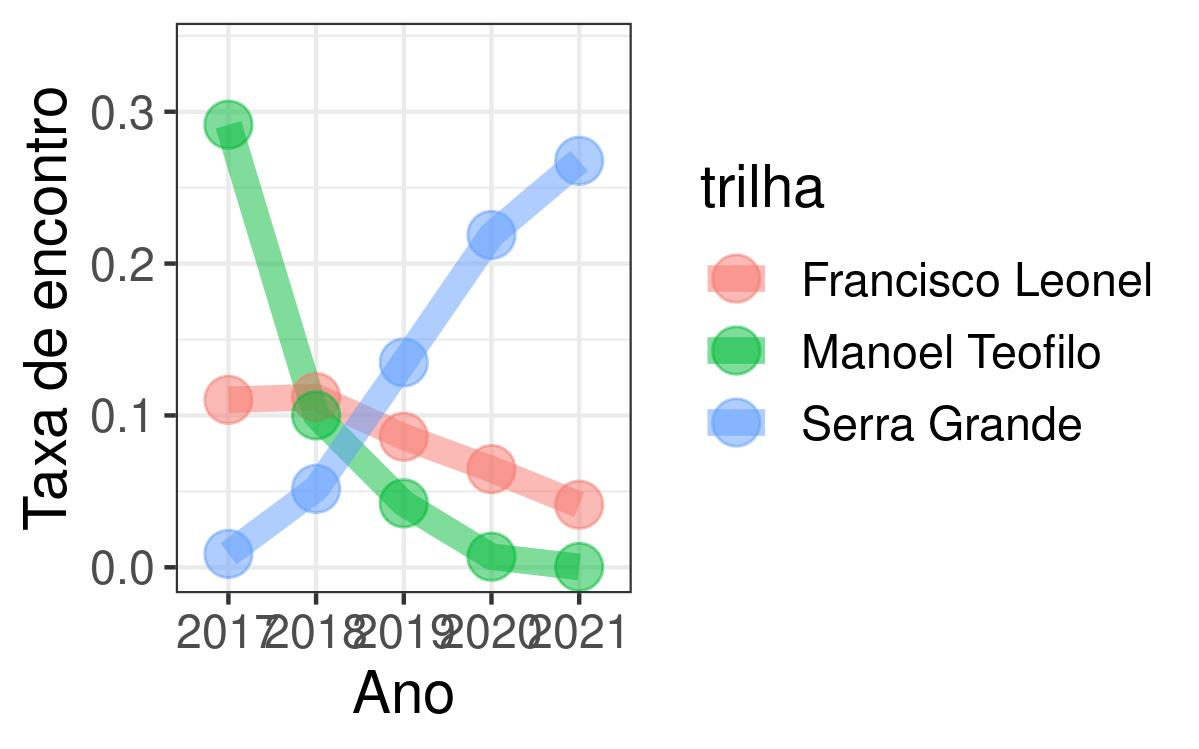
\includegraphics[width=16.65in]{/home/elildojr/Documents/r/Programa-Monitora-Florestal-Global/encontro_saberes/ouro_preto/Dasyprocta fuliginosa 2017 a 2021 por trilha} \caption[Figura 6]{Figura 6. Taxa de encontro anual para cutia por trilha na Resex do Rio Ouro Preto, 2017-2021}\label{fig:unnamed-chunk-7}
\end{figure}

Como se pode observar nas figuras acima, houve enorme variação nas
tendências populacionais entre as trilhas. Em alguns casos, elas parecem
concordar entre si. Por exemplo, os quatipurus declinaram em todas as
trilhas, embora tenha ocorrido um aumento temporário entre 2017 e 2018
na trilha Alto Caeté. A cutia declinou entre 2016 e 2017 em todas as
trilhas (mas depois disso, ela se recuperou nas trilhas Cazumbá e Gama,
mas sofreu uma nova queda na trilha Alto Caeté). O caititu declinou nas
trilhas Caeté e Gama (mas aumentou na trilha Cazumbá).

Em outros casos, as trilhas contam histórias totalmente diferentes: a
cutiara permaneceu relativamente estável na trilha Gama, declinou na
trilha Cazumbá e aumentou na trilha Alto Caeté.

\hypertarget{perguntas-e-reflexuxf5es}{%
\section{Perguntas e reflexões}\label{perguntas-e-reflexuxf5es}}

O que está acontecendo com os quatipurus? Eles estão realmente
declinando, ou as pessoas estão registrando menos por ser uma espécie
pequena, que não é caçada etc.?

De forma geral, a população de cutias parece estar estável. No entanto,
elas sofreram um tombo em 2017. O que aconteceu nesse ano? Houve algum
evento incomum, como uma seca mais forte ou algum desequilíbrio
ambiental?

A cutiara também parece ter sofrido uma queda entre 2015 e 2017, mas não
foi um tombo tão forte como o da cutia. O que será que aconteceu?

O caititu parece estar estável\ldots{} ou está declinando bem devagar ao
longo dos anos? Somente com mais anos de monitoramento poderemos saber.

Porque as tendências populacionais variaram tanto entre as trilhas?

Porque é importante monitorar várias trilhas ao invés de apenas uma?

\bibliography{skeleton.bib}



\end{document}
